% Slide file generated by /Users/e21660/shankar/bin/slides-beam from pegproof.slide

\documentclass[xcolor=dvipsnames]{beamer}

\mode<presentation>
\usetheme{Warsaw}
\usecolortheme[named=Mahogany]{structure}
\usepackage{relsize,alltt,fancybox,color}
\def\labelitemii{$\circ$}
\def\labelitemiii{$\star$}
\def\labelitemiv{$\diamond$}
\usepackage{tabularx}
\usepackage{listings}
\usepackage[english]{babel}
\usepackage[utf8]{inputenc}
\usepackage[T1]{fontenc}
\usepackage{relative}
\usepackage{tikz}
\usetikzlibrary{tikzmark}

\usepackage{listings}
%% Gestion des codes sources
\lstdefinelanguage{PVS}{
   morekeywords={AND, CONJECTURE, FACT, LET, TABLE, ANDTHEN, CONTAINING, FALSE, LIBRARY, THEN, ARRAY, CONVERSION, FORALL, MACRO, THEOREM, ASSUMING, CONVERSION+, FORMULA, MEASURE, THEORY, ASSUMPTION, CONVERSION-, FROM, NONEMPTY, TYPE, TRUE, AUTO, REWRITE, COROLLARY, FUNCTION, NOT, TYPE, AUTO, REWRITE+, DATATYPE, HAS, TYPE, O, TYPE+, AUTO, REWRITE-, ELSE, IF, OBLIGATION, VAR, AXIOM, ELSIF, IFF, OF, WHEN, BEGIN, END, IMPLIES, OR, WHERE, BUT, ENDASSUMING, IMPORTING, ORELSE, WITH, BY, ENDCASES, IN, POSTULATE, XOR, CASES, ENDCOND, INDUCTIVE, PROPOSITION, CHALLENGE, ENDIF, JUDGEMENT, RECURSIVE, CLAIM, ENDTABLE, LAMBDA, SUBLEMMA, CLOSURE, EXISTS, LAW, SUBTYPES, COND, EXPORTING, LEMMA, SUBTYPE, OF},
    sensitive=false, % keywords are not case-sensitive
    morecomment=[l]{\%}, % l is for line comment
    morestring=[b]" % defines that strings are enclosed in double quotes
}
\definecolor{gainsboro}{rgb}{0.86, 0.86, 0.86}
\lstset{keepspaces=true}
\lstset{columns=fixed}
\lstset{linewidth=.99\linewidth}
\lstset {
	basicstyle=\small\smaller\ttfamily,
	keywordstyle=\color{purple},
	commentstyle=\color{red},
	breaklines,
	breakindent=0.7em,
	backgroundcolor=\color{gainsboro},
    %numbers=left,
    tabsize=2,
    %stepnumber=1,
	frame=single,
    inputencoding=utf8,
    extendedchars=true,
	literate={\ \ }{{\ }}1 {ε}{{$\epsilon$}}1 {λ}{{$\lambda$}}1 {∀}{{$\forall$}}1 {⇒}{{$\Rightarrow$ }}1 {∧}{{$\wedge$ }}1 {∨}{{$\vee$ }}1 {Δ}{{$\Delta$}}1 {⇔}{{ $\iff$ }}1 {ω}{{$\omega$ }}1  {⊥}{{$\bot$ }}1 {⊤}{{$\top$ }}1
}
\newcommand{\lstin}[1]{\lstinline[language=PVS]{#1}}



\lstset{
    breakatwhitespace=false,
    breaklines=true,
    captionpos=b,
    keepspaces=true,
    numbersep=5pt,
    showspaces=false,
    showstringspaces=false,
    showtabs=false,
    tabsize=2,
    basicstyle=\fontsize{8.0}{9}\ttfamily,
    numbers=left,
    %xleftmargin=2em,
    framexleftmargin=1.5em,
    numberstyle=\ttfamily\tiny,
    frame = single,
    linewidth=1.02\linewidth,
    xleftmargin=.068\linewidth,
    xrightmargin=.025\linewidth,
}
\author[Natarajan Shankar]{N. Shankar}
\setbeamercolor{title}{fg=white!80!blue}
\setbeamercovered{transparent}
%\logo{\includegraphics[height=0.5cm]{/Users/shankar/images/sri_blue_logo.jpg}}
 \input{smacros}
% \newcommand{\inred}[1]{\textcolor{Red}{#1}}
% \newcommand{\ingreen}[1]{\textcolor{Green}{#1}}
% \newcommand{\htriple}[3]{\{#1\} #2 \{#3\}}
% \newcommand{\pclause}[2]{[#1 \pif #2]}
% \newcommand{\plet}[2]{\mbox{let }\ #1 \mbox{ in } #2}
% \newcommand{\ifte}[3]{\mbox{if } #1 \mbox{ then } #2 \mbox{ else } #3}
% \newcommand{\mupdate}[3]{\mathit{update}(#1, #2, #3)}
% \newcommand{\incr}[2]{\mathit{inc}(#1, #2)}
% \newcommand{\decr}[2]{\mathit{dec}(#1, #2)}
% \newcommand{\mmark}{\mathit{mark}}
% \newcommand{\bfnewint}{\mathbf{newInt}}
% \newcommand{\bfnewref}{\mathbf{newRef}}
% \newcommand{\bfpop}{\mathbf{pop}}
% \newcommand{\rlongrightarrow}{\stackrel{+}{\longrightarrow}}
% \newcommand{\rLongrightarrow}{\stackrel{+}{\Longrightarrow}}
% \newcommand{\slongrightarrow}{\stackrel{*}{\longrightarrow}}
% \newcommand{\sLongrightarrow}{\stackrel{*}{\Longrightarrow}}
% \newcommand{\dlongrightarrow}{\stackrel{\delta}{\longrightarrow}}
% \newcommand{\ttnil}{\texttt{nil}}
% \newcommand{\mvars}[1]{\mathit{mvars}(#1)}
% \newcommand{\plambda}[2]{\lambda (#1): #2}
% \newcommand{\rectype}[1]{[\# #1 \#]}
\usepackage{fancyvrb}
\usepackage[mathletters]{ucs}
%\usepackage[utf8]{inputenc}
%\DeclareUnicodeCharacter{00A0}{~}
\newcommand{\bftrue}{\mathbf{true}}
\newcommand{\bffalse}{\mathbf{false}}

\title[{\makebox[.45\paperwidth]{\greencol{Verifying PEG}

\hfill%
        \insertframenumber/\inserttotalframenumber}}]{{\textbf{Toward Robust Verification of PEG Parser Interpreters\footnote{  This work was supported by DARPA under agreement number
  HR001119C0075.  The views and conclusions contained herein are those
  of the authors and should not be interpreted as necessarily
  representing the official policies or endorsements, either expressed
  or implied, of DARPA or the U.S. Government.  Joint work with Zephyr Lucas (Dartmouth).
}}}
}
\institute{  Computer Science Laboratory\\
  SRI International\\
  Menlo Park, CA}
\date{Mar 6, 2024%\\{\small Statement A: Approved for public release; distribution is unlimited.}
}
\beamertemplatenavigationsymbolsempty
\begin{document}


\begin{frame}[plain]
\titlepage
\end{frame}

\begin{frame}[fragile]
\frametitle{Overview}
\begin{itemize}
\item The number and complexity of data and file formats is growing by the day.
\item Bad or missing input validation of the input in these formats is a major source of security vulnerabilities.
\item The Parsley data definition language is a way of specifying such language formats based on
\begin{enumerate}
\item Parsing Expression Grammars (PEGs) as the basic grammar definition
\item Attribute grammars for capturing data dependencies using inherited and synthesized attributes over PEG grammars
  \item A functional language for defining computations and constraints. 
\end{enumerate}
\item The talk focuses on the PEG aspect of Parsley with a verification and proof of, and code extraction from,
a parsing abstract machine for PEGs.
\end{itemize}
\end{frame}


\begin{frame}[fragile]
\frametitle{Managing the Proof Lifecycle}
\begin{itemize}
\item The 1992 CADE paper introducing PVS captures the motivation for many of the design choices in PVS
for supporting the scalable construction of robust proofs: 
{\small\smaller\smaller
  \begin{quote}
  \emph{Our experience with mechanical verification of complex
    designs and algorithms has led us to conclude that, just as with software, there is a lifecycle
    to a mechanically-checked proof. In the initial exploratory phase of proof development, we are
    mainly interested in debugging the specification and putative theorems, and in testing and
    revising the key, high-level ideas in the proof. An important requirement in this phase is early
    and useful feedback when a purported theorem is, in fact, false. Once the basic intuitions have
    been acquired and the formalization is stable, the proof checking enters a development phase
    where we take care of the details and construct the proof in larger leaps. Efficiency of proof
    development is a key requirement here. In the third, presentation phase,the proof is honed and
    polished for presentation in order to be scrutinized by the social process.  Readability and
    intellectual perspicuity of the output is the goal here. The final phase is generalization where
    we carefully analyze the finished proof, weaken and generalize the assumptions, extract the key
    insights and proof techniques,and make it easier to carry out subsequent verifications of a
    similar nature.  Maintenance is a special application of generalization, where we adapt a
    verification to slightly changed assumptions or requirements.  Robustness of the proof procedure
    is a useful attribute here.  }
  \end{quote}
}
\end{itemize}
\end{frame}


\begin{frame}[fragile]
\frametitle{The PVS Language in Brief}
\begin{itemize}
\item %\pause
{\small\smaller A PVS specification is a collection of libraries.
\begin{itemize}
\item Each library is a collection of files.
  \item Each file is a sequence of theories.
    \item Each theory is a sequence of declarations/definitions of types, constants, and formulas (Boolean expressions).
    \end{itemize}
}
%\pause    
\item {\small\smaller Types include
\begin{enumerate}
\item Booleans, number types
\item Predicate subtypes: $\{x : T | p(x)\}  $ for type $T$ and predicate $p$. 
\item Dependent function $[x: D \rightarrow R(x)]$, tuple $[x : T_1, T_2(x)]$, and record $[\# a: T_1, b: T_2(x) \#]$ types.
\item Algebraic and coalgebraic datatypes: lists, trees, ordinals. 
\end{enumerate}
}
%\pause
\item {\small\smaller Expressions in PVS are
\begin{enumerate}
\item Booleans, numbers
\item Application : $f(a_1, \ldots, a_n)$
\item Abstraction : $\lambda (x_1: T_1, \ldots, x_n: T_n): a$
\item Tuples: $(a_1, \ldots, a_n)$, $a`3$
\item Records: $({\small \#} l_1:= a_1, \ldots, l_n := a_n {\small \#})$, $a`l_i$
\item Conditionals: $\mbox{IF } {a_1} \mbox{ THEN } {a_2} \mbox{ ELSE } {a_3} \mbox{ ENDIF}$
\item Updates: $a~\mathtt{WITH}~[(3)`1`age := 37]$.    
\end{enumerate}}
\end{itemize}
\end{frame}


\begin{frame}[fragile]
\frametitle{Code Generation from a Specification Language: PVS2CL}
\begin{itemize}
\item Quantification and equality over higher types are not executable, but many definitions are. 
\item Mapping PVS to Common Lisp is relatively direct: each construct is mapped to its Lisp counterpart
and types are transformed in to compiler declarations. 
\item Array, record, tuple updates are a bit challenging: need to
minimize copying by performing destructive updates.  
\item PVS2CL uses a static analysis to identify whether a reference is live in the context of
its update.\footnote{Shankar, N.: Static analysis for safe destructive updates in a functional language, LOPSTR 2001.}
\item %\pause
\rdmph{Code generation is different from implementation --- can't create a bespoke runtime.}
\item \rdmph{A (principled) specification logic like PVS is not a (pragmatic) programming language. }
\item \bluemph{Executable specifications are very useful for animation, testing, validation, proof, and system building.}
\end{itemize}
\end{frame}


\begin{frame}[fragile]
\frametitle{Functional vs. Imperative}
\begin{itemize}
\item Functional and imperative languages are quite different, both syntactically and semantically. 
\item %\pause
With functional languages 
\begin{itemize}
\item Referentially transparency is a key property
\item Both manual and mechanical verification are more civilized
\item Evaluation is pure (updates are nondestructive)
\item  Memory management is implicit.
\end{itemize}
\item %\pause
With imperative languages
\begin{itemize}
\item Scoping is tricky:  No counterpart of let-expressions in many imperative languages
\item Evaluation is triggered by control flow not value flow
\item Semantically closer to machine execution
\item Integrated with extensive libraries and application software
\item Memory management may be explicit, e.g., through \texttt{free} and \texttt{malloc}. 
\end{itemize}
\end{itemize}
\end{frame}


\begin{frame}[fragile]
\frametitle{The PVS2C Code Generator}
\begin{itemize}
\item PVS2C generates safe, efficient, standalone C code for a full functional fragment of PVS.
\item Each PVS theory \texttt{foo.pvs} generates a \texttt{foo.h} and \texttt{foo.c}.\footnote{\smaller\smaller F\'erey, G., Sh\_, N.: Code Generation using a formal model of reference counting, NFM 2016.  See also Wolfram Schulte, 
 Deriving reference count garbage collectors,  {\em 6th International Symposium on Programming Language
  Implementation and Logic Programming}, 1994.}
}
\item The translation is factored through an intermediate language that represents PVS expressions in A-normal form and
performs a light static analysis to identify the \emph{release points} for references.
\begin{center}
  \includegraphics[width=.9\linewidth]{/Users/e21660/shankar/projects/PVSCodeGen/Figures/pvs2c.png}
\end{center}
\end{itemize}
\end{frame}


\begin{frame}[fragile]
\frametitle{PVS2C: Putting Theory to Use}
\begin{itemize}
\item The theoretical outline above deals with an idealized first-order language with
(unbounded) integers and arrays.  
\item %\pause
The full PVS2C implementation covers
\begin{enumerate}
\item Multi-precision rational numbers and integers, and floats
\item Fixed-size arithmetic: \texttt{uint8}, \texttt{uint16}, \texttt{uint32}, \texttt{uint64}, \texttt{int8}, \texttt{int16}, \texttt{int32}, \texttt{int64}, with safe casting  
\item Dependent (dynamically sized) and infinite arrays 
\item Dependent records and tuples
\item Higher-order functions and closures (with updates) 
\item Characters (ASCII and Unicode)  and strings  
\item Algebraic datatypes
\item Parametric theories with type parameters (unboxed polymorphism)
\item Memory-mapped File I/O
\item Semantic attachments
\item JSON representation for data
\end{enumerate}
\item %\pause
PVS2C captures a functional subset of PVS that is usable as a safe programming language
- a well-typed program cannot fail (modulo resource limitations).
\end{itemize}
\end{frame}


\begin{frame}[fragile]
\frametitle{Experiments in Code Generation: HMAC from Wikipedia}
{\small\smaller\smaller \begin{smallersession}
function hmac is
    input:
        key:        Bytes    // Array of bytes
        message:    Bytes    // Array of bytes to be hashed
        hash:       Function // The hash function to use (e.g. SHA-1)
        blockSize:  Integer  // The block size of the hash function 
                                           //(e.g. 64 bytes for SHA-1)
        outputSize: Integer  // The output size of the hash function 
                                           //(e.g. 20 bytes for SHA-1)

    // Keys longer than blockSize are shortened by hashing them
    if (length(key) > blockSize) then
        key <- hash(key) // key is outputSize bytes long

    // Keys shorter than blockSize are padded to blockSize by padding 
    //with zeros on the right
    if (length(key) < blockSize) then
        key <- Pad(key, blockSize) // Pad key with zeros to make it
                                   // blockSize  bytes long
    o_key_pad <- key xor [0x5c * blockSize]   // Outer padded key
    i_key_pad <- key xor [0x36 * blockSize]   // Inner padded key
    return hash(o_key_pad \(\|\) hash(i_key_pad \(\|\) message))
  \end{smallersession}}

\end{frame}


\begin{frame}[fragile]
\frametitle{HMAC in PVS}
  \begin{smallersession}
{\smaller    
hmac(blockSize: uint8,
     key : bytestring,
     (message : bytestring |
        message`length + blockSize < bytestring_bound),
     outputSize: upto(blockSize),
     hash: [bytestring->lbytes(outputSize)]): lbytes(outputSize)
= LET newkey = IF length(key) > blockSize THEN hash(key) ELSE key ENDIF,
      newerkey: lbytes(blockSize)
       = IF length(newkey) < blockSize
          THEN padright(blockSize)(newkey)
          ELSE newkey
         ENDIF, 
      oKeyPad = lbytesXOR(blockSize)(newerkey, nbytes(0x5c, blockSize)),
      iKeyPad = lbytesXOR(blockSize)(newerkey, nbytes(0x36, blockSize))
   IN hash(oKeyPad ++ hash(iKeyPad ++ message))

hmac256((blockSize: uint8 | 32 <= blockSize),
        key : bytestring,
        (message : bytestring | 
             message`length + blockSize < bytestring_bound))
      : lbytes(32)
= hmac(blockSize, key, message, 32, sha256message)    
}    \end{smallersession}

\end{frame}


\begin{frame}[fragile]
\frametitle{HMAC Generated by PVS2C}
{\tiny\smaller    \begin{smallersession}
    bytestrings__bytestring_t
    HMAC__hmac256(uint8_t ivar_2, bytestrings__bytestring_t ivar_3,
                  bytestrings__bytestring_t ivar_4)\{
        bytestrings__bytestring_t  result;
        uint8_t ivar_18;
        ivar_18 = (uint8_t)32;
        HMAC_funtype_0_t ivar_19;
        HMAC_closure_3_t cl1230;
        cl1230 = new_HMAC_closure_3();
        ivar_19 = (HMAC_funtype_0_t)cl1230;
        bytestrings__bytestring_t ivar_14;
        ivar_14 = (bytestrings__bytestring_t)
        HMAC__hmac((uint8_t)ivar_2, (bytestrings__bytestring_t)ivar_3,
                   (bytestrings__bytestring_t)ivar_4, (uint8_t)ivar_18,
                   (HMAC_funtype_0_t)ivar_19);
        //copying to bytestrings__bytestring
        //from bytestrings__bytestring;
        result = (bytestrings__bytestring_t)ivar_14;
        if (result != NULL) result->count++;
        release_bytestrings__bytestring(ivar_14);
        return result;
\}
\end{smallersession}}

\end{frame}


\begin{frame}[fragile]
\frametitle{Parsing Expression Grammars (PEG)}
\begin{itemize}
\item PEG grammars are a natural class that capture \emph{recursive descent}
parsers.
\item The constructs and their semantics are shown below.  $\sigma \models e, \sigma'$ means that
the expression $e$ recognizes $\sigma$ leaving a (unique) suffix $\sigma'$.  Otherwise, $\sigma\not\models e$\@.  
\begin{enumerate}
\item Empty: $\varepsilon$, where $\sigma \models \varepsilon, \sigma$
\item Terminal: $c$, where $c\sigma \models c, \sigma$
  \item Any: $\mathit{any}$, where $c\sigma \models \mathit{any}, \sigma$
\item Ordered choice: $E_1/E_2$, where $\sigma \models E_1/E_2, \sigma'$ iff $\sigma\models E_1, \sigma'$ or if $\sigma\not\models E_1$ and $\sigma\models E_2, \sigma'$
\item Iteration: $E^*$ and $E^+$ where $\sigma\models E^*, \sigma'$ iff $\sigma\not\models E$ and $\sigma' = \sigma$ or $\sigma\models E, \sigma''$ and $\sigma''\models E^*, \sigma'$
\item Optional: $E?$, where $E\models E?, \sigma'$ iff $\sigma\models E, \sigma'$ or $\sigma' = \sigma$
\item And:$\& E$, where $\sigma\models \& E, \sigma$ iff $\sigma \models E, \sigma'$ for some $\sigma'$
\item Negation: $!E$, where $\sigma \models !E, \sigma$ iff $\sigma\not\models E$
\end{enumerate}
\item Example: The non-CFG expression $a^nb^nc^n$ is PEG-expressible, but the exact relationship between PEGs and CFG is open.  
%Undecidable PEG problems include equivalence, empty string acceptance, emptiness, and termination.
\end{itemize}
\end{frame}


\begin{frame}[fragile]
\frametitle{PEG Grammars in PVS (with Clement Blaudeau, CPP'20)}
\begin{itemize}
\item PEG expressions are formalized as an algebraic datatype in PVS.  
\item A PEG grammar assigns PEG expressions $e$ to  nonterminals $N$: $N \leftarrow e$. 
\item Not all such grammars are well-formed since direct or indirect
left-recursive rules would lead to nonterminating parsers, e.g., $S \leftarrow S/a$
is ill-formed. 
\item The grammar rules are statically analyzed for well-formedness.
\item Na\"{\i}ve PEG parsing can be inefficient since the tests ($E?$,
$\&E$, $!E$) and ordered choice ($E_1/ E_2$) can involve repeated
parsing of substrings for the same nonterminal.'
\end{itemize}
\end{frame}


\begin{frame}[fragile]
\frametitle{Formalizing PEG Parsing in PVS}
\begin{itemize}
\item We have formalized the metatheory of PEG grammars in PVS.
\item We defined a static analysis on PEG grammars to identify whether
a PEG expression can possibly fail, possibly succeed without consuming any input, or
 succeed only by consuming some input.
\item This is used to define a reference PEG parser and prove its termination, e.g., by constraining 
a rule $N\leftarrow e$ so that $e$ must contain only smaller nonterminals in positions that can be reached (through success or failure) without consuming input.
\item This check is necessarily conservative since termination of PEG grammars is undecidable.  
\item Well-formed grammars yield a terminating parser that constructs a parse tree. 
\item The parse tree datatype captures the \emph{proof of parse-correctness}, including
proof of failure.
% We have verified PEG packrat parsers without and with semantic actions in PVS. 
\end{itemize}
\end{frame}


\begin{frame}[fragile]
\frametitle{Chart Parsing of PEGs }
\begin{itemize}
\item Our PEG expression language consists of productions in Chomsky Normal Form:
\begin{center}
\begin{tabular}{{|l|c|}}\hline
  Empty &   $A \leftarrow \epsilon$ \\\hline
  Failure & $A \leftarrow f$ \\\hline
  Any & $A \leftarrow .$ \\\hline
  Terminal & $A \leftarrow c$ \\\hline
  Concatenation & $A \leftarrow B~C$ \\\hline
  Ordered Choice & $A \leftarrow B/C$ \\\hline
  Check & $A \leftarrow \& B$ \\\hline
  Negation & $A \leftarrow !B$ \\\hline
\end{tabular}
\end{center}
\item Grammars associate a PEG expression with each nonterminal --- unlike the previous proof, there is no static
analysis for well-formed grammars; loops are detected dynamically during parsing.
\end{itemize}
\end{frame}


\begin{frame}[fragile]
\frametitle{An Example}
\begin{itemize}
\item   We want to parse (a prefix of) strings with linearly nested matched parentheses: \texttt{(((\ldots)))}.
\item   The grammar and initial scaffold are shown below (with '{?}' for pending):
$$
\begin{array}[c]{|c|c|c|c|c|c|}\hline
  & \multicolumn{5}{c|}{Position} \\\hline
NT  & 0 \mbox{\lq\texttt{(}\rq}& 1 \mbox{\lq\texttt{(}\rq}& 2 \mbox{\lq\texttt{)}\rq}& 3 \mbox{\lq\texttt{)}\rq} & 4 \\\hline\hline
S \leftarrow  P / E &  ? & ? & ? & ? & ? \\\hline
  P \leftarrow  \mathit{BP}~\mathit{CP}    &  ? & ? & ? & ? & ? \\\hline
  CP \leftarrow  S~\mathit{EP} &  ? & ? & ? & ? & ? \\\hline
  BP \leftarrow \textit{ term}(\mbox{\lq\texttt{(}\rq}) &  ? & ? & ? & ? & ? \\\hline
  EP \leftarrow  \textit{term}(\mbox{\lq\texttt{)}\rq}) &  ? & ? & ? & ? & ? \\\hline
  E \leftarrow  \varepsilon  & ? & ? & ? & ? & ? \\\hline    
\end{array}
$$
\end{itemize}
\end{frame}


\begin{frame}[fragile]
\frametitle{Example: Unfolding the Start Query}
\begin{itemize}
\item We evaluate the top query $(S, 0)$, i.e., parse nonterminal $S$ at nonterminal $0$, where
$\mathbf{p}(\phi, 0)$ represents the null stack, and $\mathbf{p}(S, 0)$ indicates the next stack position is $a(0)(S)$\@.  
$$
\begin{array}[c]{|c|c|c|c|c|c|}\hline
  & \multicolumn{5}{c|}{Position} \\\hline
NT  & 0 \mbox{\lq\texttt{(}\rq}& 1 \mbox{\lq\texttt{(}\rq}& 2 \mbox{\lq\texttt{)}\rq}& 3 \mbox{\lq\texttt{)}\rq} & 4 \\\hline\hline
S \leftarrow  \fbox{P} / E &  \mathbf{p}(\phi, 0)\tikzmark{a1} & ? & ? & ? & ? \\\hline
  P \leftarrow  \mathit{\fbox{BP}}~\mathit{CP}    &  \mathbf{p}(S, 0)\tikzmark{b1} & ? & ? & ? & ? \\\hline
  CP \leftarrow  S~\mathit{EP} &  ? & ? & ? & ? & ? \\\hline
  BP \leftarrow \textit{ term}(\mbox{\lq\texttt{(}\rq}) &  \mathbf{p}(P, 0)\tikzmark{c1} & ? & ? & ? & ? \\\hline
  EP \leftarrow  \textit{term}(\mbox{\lq\texttt{)}\rq}) &  ? & ? & ? & ? & ? \\\hline
  E \leftarrow  \varepsilon  & ? & ? & ? & ? & ? \\\hline    
\end{array}
$$
\begin{tikzpicture}[overlay, remember picture, yshift=.25\baselineskip, shorten >=.5pt, shorten <=.5pt]
    \draw [->] ({pic cs:b1}) [bend right] to ({pic cs:a1});
    \draw [->] ({pic cs:c1})[bend right] to ({pic cs:b1});
  \end{tikzpicture}
\end{itemize}
\end{frame}


\begin{frame}[fragile]
\frametitle{Example: Unwinding the Parse}
\begin{itemize}
\item We evaluate the top query $(S, 0)$, i.e., parse nonterminal $S$ at nonterminal $0$, where
$\mathbf{p}(\phi, 0)$ represents the null stack, and $\mathbf{p}(S, 0)$ indicates the next stack position is $a(0)(S)$\@.  
$$
\begin{array}[c]{|c|c|c|c|c|c|}\hline
  & \multicolumn{5}{c|}{Position} \\\hline
NT  & 0 \mbox{\lq\texttt{(}\rq}& 1 \mbox{\lq\texttt{(}\rq}& 2 \mbox{\lq\texttt{)}\rq}& 3 \mbox{\lq\texttt{)}\rq} & 4 \\\hline\hline
S \leftarrow  \fbox{P} / E &  \mathbf{p}(\phi, 0)\tikzmark{a2} & \mathbf{p}(CP, 1)\tikzmark{e2} & ? & ? & ? \\\hline
  P \leftarrow  {\mathit{\fbox{BP}}}~\mathit{\fbox{CP}}    &  \mathbf{p}(S, 0)\tikzmark{b2} & \mathbf{p}(S, 1)\tikzmark{f2} & ? & ? & ? \\\hline
  CP \leftarrow  \fbox{S}~\mathit{EP} &  ? & \mathbf{p}(P, 0)\tikzmark{d2} & ? & ? & ? \\\hline
  BP \leftarrow \textit{ term}(\mbox{\lq\texttt{(}\rq}) &  \mathbf{g}(0, 1)\tikzmark{c2} & \mathbf{p}(P, 1)\tikzmark{g2} & ? & ? & ? \\\hline
  EP \leftarrow  \textit{term}(\mbox{\lq\texttt{)}\rq}) &  ? & ? & ? & ? & ? \\\hline
  E \leftarrow  \varepsilon  & ? & ? & ? & ? & ? \\\hline    
\end{array}
$$
\begin{tikzpicture}[overlay, remember picture, yshift=.25\baselineskip, shorten >=.5pt, shorten <=.5pt]
    \draw [->] ({pic cs:b2}) [bend right] to ({pic cs:a2});
    \draw [->] ([xshift=-1.2cm]{pic cs:d2})[bend right] to ({pic cs:b2});
    \draw [->] ([yshift=3pt]{pic cs:e2})[bend left] to ({pic cs:d2});
    \draw [->] ({pic cs:f2})[bend right] to ({pic cs:e2});
    \draw [->] ({pic cs:g2})[bend right] to ({pic cs:f2});    
  \end{tikzpicture}
\end{itemize}
\end{frame}


\begin{frame}[fragile]
\frametitle{Example: Completing the Parse}
\begin{itemize}
\item The scaffold for the full parse is thus filled out with entries as shown below. 
$$
\begin{array}[c]{|c|c|c|c|c|c|}\hline
  & \multicolumn{5}{c|}{Position} \\\hline
NT  & 0 \mbox{\lq\texttt{(}\rq}& 1 \mbox{\lq\texttt{(}\rq}& 2 \mbox{\lq\texttt{)}\rq}& 3 \mbox{\lq\texttt{)}\rq} & 4 \\\hline\hline
S \leftarrow  P / E &  \mathbf{g}(7, 4) & \mathbf{g}(4, 2) & \mathbf{g}(1, 0) & ? & ? \\\hline
  P \leftarrow  \mathit{BP}~\mathit{CP}  &  \mathbf{g}(6, 4) & \mathbf{g}(3, 2) & \mathbf{f}(1) & ? & ? \\\hline
  CP \leftarrow  S~\mathit{EP} &  ? & \mathbf{g}(5, 3) & \mathbf{g}(2, 1) & ? & ? \\\hline
  BP \leftarrow \textit{ term}(\mbox{\lq\texttt{(}\rq}) &  \mathbf{g}(0, 1) & \mathbf{g}(0, 1) & \mathbf{f}(0) & ? & ? \\\hline
  EP \leftarrow  \textit{term}(\mbox{\lq\texttt{)}\rq}) &  ? & ? & \mathbf{g}(0, 1) & \mathbf{g}(0, 1) & ? \\\hline
  E  \leftarrow  \varepsilon   & ? & ? & \mathbf{g}(0, 0) & ? & ? \\\hline
\end{array}
$$
\end{itemize}
\end{frame}


\begin{frame}[fragile]
\frametitle{(Chomsky-normal form) PEGs in PVS}
  \begin{smallersession}
len, max: VAR index %the length of the input
byte: TYPE = below(256)
strings(len): TYPE = ARRAY[below(len) -> byte]
num_non_terminals: byte = 255
non_terminal: TYPE = below(num_non_terminals)

peg  : DATATYPE
  BEGIN
   epsilon : epsilon?
   failure : failure?
   any(p : [byte -> bool]) : any?
   terminal(a: byte) : terminal?
   concat(e1, e2: non_terminal) : concat?
   choice(e1, e2: non_terminal) : or?
   check(e: non_terminal) : and?
   neg(e: non_terminal) : not?
  END peg
\end{smallersession}

\end{frame}


\begin{frame}[fragile]
\frametitle{The Scaffold}
The scaffold is a two-dimensional array mapping each position/nonterminal to an entry.
\begin{smallersession}
scaffold(len) : TYPE
= ARRAY[pos: upto(len) ->
    ARRAY[non_terminal -> (nice_entry?(len, pos))]]  
\end{smallersession}
$$
\begin{array}{|r||c|c|c|c|c|}\hline
  & 0 & \ldots & i & \ldots & L \\\hline\hline
  n0 & a_{00}& \ldots & a_{i0}\tikzmark{a} & \ldots & a_{L0}\\\hline
  \vdots & \vdots & \vdots & \vdots & \vdots & \vdots\\\hline
  nj & \ldots & \ldots & a_{ij}\tikzmark{b} & \ldots & a_{Lj}\\\hline
  \vdots & \vdots & \vdots & \vdots & \tikzmark{c}\vdots & \vdots\\\hline  
  nN & a_{0N}& \ldots & a_{iN} & \ldots & a_{LN}\\\hline
\end{array}
$$
\begin{tikzpicture}[overlay, remember picture, yshift=.25\baselineskip, shorten >=.5pt, shorten <=.5pt]
    \draw [->] ({pic cs:b}) [bend right] to ({pic cs:a});
    \draw [->] ([yshift=.75pt]{pic cs:b}) -- ({pic cs:c});
  \end{tikzpicture}

\end{frame}


\begin{frame}[fragile]
\frametitle{Step Function}
  \begin{smallersession}
step(len, G, (s: strings(len)), (start: upto(len)),
     (rootnt: non_terminal))
    (St : state(len, G, s, start, rootnt))
    : state(len, G, s, start, rootnt)
 = (LET scaf = St`scaf,
	stack = St`stack,
	depth = St`depth,
	lflag = St`lflag
     IN
    IF empty?(stack)
    THEN St
    ELSE LET pos = pos(stack),
             cur = nt(stack),
	     rest = scaf(pos)(cur)
	  IN CASES G(cur) OF
          epsilon: St WITH [`scaf(pos)(cur) := good(0, 0),
                            `stack := rest,
                            `depth := depth - 1],
    \vdots
  \end{smallersession}

\end{frame}


\begin{frame}[fragile]
\frametitle{Outer Parsing Loop}
  \begin{smallersession}
    parse(len, G, (s: strings(len)), (start: upto(len)),
           (root: non_terminal), St : state(len, G, s, start, root))
    : RECURSIVE endstate(len, G, s, start, root)
  = (IF St`depth = 0
      THEN St
      ELSE parse(len, G, s, start, root,
                 step(len, G, s, start, root)(St))
      ENDIF)
      MEASURE size(len, G, s, start, root)(St) BY <
    \end{smallersession}

\end{frame}


\begin{frame}[fragile]
\frametitle{Proof-of-Parse Verification    }
    Defined a proof-of-parse format for success, failure, loop outcomes and extracted valid proofs from parser output.
\begin{smallersession}
  buildproof(len, G, (s: strings(len)),
              (rootpos: upto(len)), (rootnt: non_terminal))
            (st: endstate(len, G, s, rootpos, rootnt),
              n, (i | i <= len)): 
     \{P | good_parsetree?(len, G, s)(qempty, n, i, P)
           AND entry(P) = st`scaf(i)(n)\}
  = (IF loop?(st`scaf(i)(n))
     THEN  (LET pendfun = (LAMBDA (n: non_terminal): pending),
                      A = (LAMBDA (i: upto(len)): pendfun)
             IN buildloop(len, G, s, rootpos, rootnt)
                         (st, A, qempty, n, i))
     ELSE buildtree(len, G, s, rootpos, rootnt)(st, qempty, n, i)
     ENDIF)

    \end{smallersession}

\end{frame}


\begin{frame}[fragile]
\frametitle{Introducing \texttt{let-then-else}}
    Even with memoization (packrat parsing), the PEG grammar can be slow because it is not backtracking efficiently from failure.


    A variant \texttt{let x = A then B else C} can be used more efficiently and replaces several PEG constructors.
    \begin{smallersession}
prepeg: DATATYPE
BEGIN
   epsilon : epsilon?
   failure : failure?
   any(p : [byte -> bool]) : any?
   terminal(a: byte) : terminal?
   lte(fst: non_terminal, lthen : non_terminal, lelse: non_terminal)
     : lte? 
END prepeg

    \end{smallersession}

    The original proofs were hard: took around four to six weeks with over a 150 nontrivial proof obligations.  

    Proofs replayed robustly even though the change was significant.

    But the speed-up was only around 30\%

\end{frame}


\begin{frame}[fragile]
\frametitle{Extending the Base Case to DFAs}
    One source of slowness is that the base case handles only one character at a time.

    The proposed remedy was to make the base case cover any DFA.
    (This is tricky DFA and PEG semantics are not compatible.)

    \begin{smallersession}
prepeg: DATATYPE
BEGIN
   epsilon : epsilon?
   failure : failure?
   any(dfa : dfa) : any?
   terminal(a: byte) : terminal?
   lte(fst: non_terminal, lthen : non_terminal, lelse: non_terminal)
     : lte? 
END prepeg
\end{smallersession}

With this, the parsing time is halved.

\end{frame}


\begin{frame}[fragile]
\frametitle{Proof Robustness}
\begin{itemize}
\item Change is the only constant.
\item No special effort was made to make the above proofs robust.
\item The pre-packaged automation (built-ins and strategies) made the proofs reusable across similar proof obligations and across the evolution of the specification/algorithm.
\item There are many sources of non-robustness:
\begin{enumerate}
\item Proof commands that mention formula numbers are sensitive to  reordering/shifting of formulas in a sequent
\item Proof commands that include expressions are sensitive to changes in these expressions, e.g., Skolem names.
\item If the order of cases changes, then proofs can lose synchrony.
  \item If definitions change, the proof obligations can get detached from their proofs. 
  \end{enumerate}
\item   A lot of post-processing is needed to define proof strategies and refactor proofs to make them robust.
\end{itemize}
\end{frame}


\begin{frame}[fragile]
\frametitle{Conclusions}
\begin{itemize}
\item   Parsing is a key gatekeeper for software systems; parsing verification needs to be streamlined.
\item   More generally, beyond data formats, modeling dominates the software development activity for critical systems.
\item   Refinement and code generation bridge the semantic gap between models and code.
\item   Robust proofs make it easier to evolve better models and implementations. 
\item   The efficiency of code generated from verified high-level models can be competitive with \emph{hand-written code}.
\item Code generation can be used to create standalone components or define entire systems.
\item \bluemph{The key value proposition is the use of one unified system and language for
  specification, modeling, programming, and proof.  }
\end{itemize}
\end{frame}

\end{document}
